\documentclass[../main.tex]{subfiles}

\begin{document}
\begin{problema}[3]
	Una deformación homogénea se define por desplazamientos que son funciones
	lineales en las coordenadas de los puntos materiales. Encuentre la forma
	original de una superficie que después de una deformación homogénea adopta
	una forma esférica.

	\startsolution

	La superficie esférica en la configuración actual puede escribirse como:

	\begin{equation}
		\norm{\vect{x}}^{2} = r^{2},
		\label{eq:spherical_surface}
	\end{equation}

	tal que

	\begin{equation}
		\vect{x} = r \vect{m},
		\label{eq:point_on_sphere}
	\end{equation}

	con \(r > 0\) y \(\vect{m} \cdot  \vect{m} = 1\).

	Antes de la deformación, en la configuración de referencia, un punto
	está dado por:

	\begin{equation}
		\vect{X} = \bm{F}^{-1}\vect{x}.
		\label{eq:point_reference_config}
	\end{equation}

	Es decir,

	\begin{figure}[htb]
		\centering
		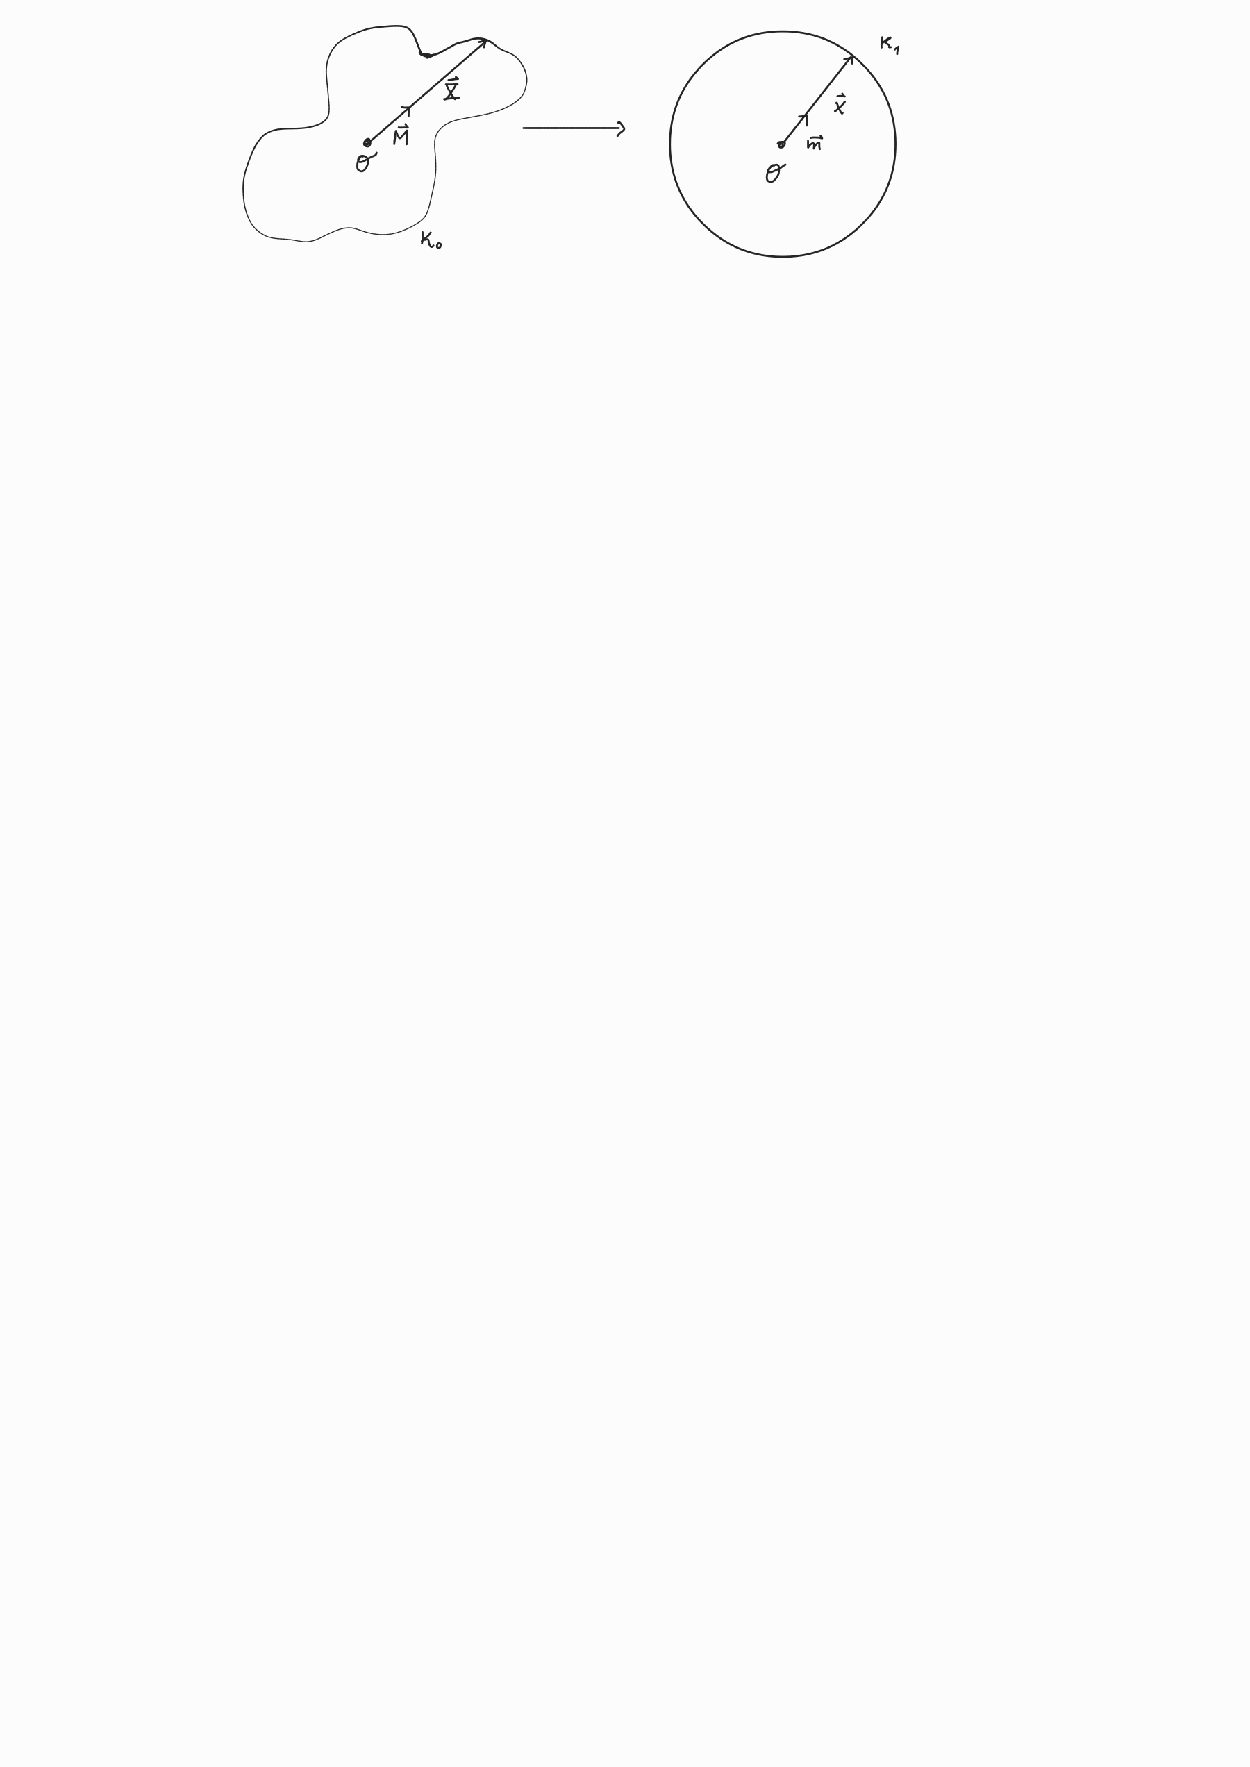
\includegraphics[scale=0.7, trim={4cm 25cm 5.2cm 0cm}, clip]{figs/problema02.pdf}
		\caption{Cuerpo en la configuración de referencia antes de conocer su forma original y cuerpo
			en la configuración actual resultado de una deformación homogénea.}
	\end{figure}

	Y puesto que para este tipo de deformaciones sabemos que los desplazamiento son
	funciones lineal, i.e.

	\begin{equation}
		\lambda \vect{M} = \bm{F}^{-1}\vect{m}.
		\label{eq:deformation_lineal}
	\end{equation}

	Entonces, por las \zcref{eq:point_on_sphere, eq:point_reference_config, eq:deformation_lineal},

	\begin{align*}
		\vect{X} & = \bm{F}^{-1}(r \vect{m}), \\
		\vect{X} & = r\lambda \vect{M}.
	\end{align*}

	Calculando el producto punto consigo mismo, recordando que \(\lambda^{2} = \vect{M} \bm{C}\vect{M}\) con
	\(\bm{C}\) el tensor derecho de Cauchy-Green, obtenemos que

	\begin{equation*}
		\vect{X}\bm{C}\vect{X} = r^{2}.
	\end{equation*}

	Además, notemos que

	\begin{equation*}
		\vect{X} = X_{i}\vect{M}_{i},
	\end{equation*}

	donde \(\{\vect{M}_{i}\}\) forman una base ortonormal.

	Escribiendo \(\bm{C}\) como

	\begin{equation*}
		\bm{C} = \sum_{i = 1}^{3}\lambda_{i}^{2} \vect{M}_{i} \otimes \vect{M}_{i}.
	\end{equation*}

	Entonces, de los resultados anteriores, obtenemos que

	\begin{equation*}
		\vect{X} \bm{C}\vect{X} = \lambda_{i}^{2}\vect{X^{\prime}}_{i}^{2},
	\end{equation*}

	tal que,

	\begin{equation*}
		\lambda_{1}^{2}X_{1}^{2} + \lambda_{2}^{2}X_{2}^{2} + \lambda_{3}^{2}X_{3}^{2} = r^{2}
	\end{equation*}

	la cual es la ecuación que describe a un elipsoide.
\end{problema}
\end{document}
